\documentclass[a4paper,12pt]{article}
\usepackage[T1]{fontenc}
\usepackage[utf8]{inputenc}
\usepackage{lmodern}
\usepackage{listings}
%\usepackage{graphicx}
\lstset{literate={í}{{\'i}}0 {ç}{{\c{c}}}1 {ã}{{\~{a}}}1 {é}{{\'e}}0 {á}{{\'a}}0 {ú}{{\'u}}1, breaklines=true}
\usepackage[simplified]{pgf-umlcd}
\usepackage[a4paper,textwidth=8in]{geometry}
\usepackage{hyperref}

\title{Aplicação do Padrão de Projeto \textit{Facade} para Implementação de um Software Auxiliar de Atividades Técnicas em Laboratórios de Química}
\author{Caio Cardoso S. G. Souza - 11814871}

\begin{document}
  \maketitle
  \section{O Padrão de Projeto \textit{Facade}}
    \subsection{Intenção e objetivo}
      O principal objetivo do padrão \textit{Facade} é fornecer uma interface unificada por meio de um conjunto para um subsistema, tornando o sistema mais fácil de usar.
    \subsection{Outros nomes conhecidos para o padrão}
      Não há outro nome amplemente usado para o padrão \textit{Facade}
    \subsection{Motivação}
      A motivação do padrão \textit{Facade} surge da complexidade em sistemas grandes que possuam diversos subsistemas. Conforme os subsistemas crescem eles tendem a ficarem mais complexos, os tornando mais difíceis ao usuário. Uma fachada então é inserida para fornecer uma interface única e simplificada para as funcionalidades gerias dos subsistemas, minimizando assim a comunicação e as dependências entre esses subsistemas.
    \subsection{Aplicabilidade}
      O padrão \textit{Facade} é recomendado para as seguintes ocasiões:
      \begin{itemize}
        \item Fornecer uma interface simples para um sibsistema complexo;
        \item Existem muitas dependências entre os clientes e as classes de implementação de uma abstração;
        \item Organizar os subsistemas em camadas, onde cada fachada define o ponto de entrada dos subsistemas;
      \end{itemize}
    \subsection{Estrutura}
      A estrutura do padrão \textit{Facade} é bem simples: é complesta pela classe de fachada e pelas classes do subsistema. A fachada sabe quais classes do subsistema são responsáveis por determinadas tarefas e delega as requisições; já as classes do subsistema compõem o subsistema em si e não possuem conhecimento da fachada.
    \subsection{Participantes}
      Como explicado no tópico anterior, o padrão \textit{Facade} possui dois tipos de participantes:
      \begin{enumerate}
        \item Fachada
        \item Classes do subsistema
      \end{enumerate}
    \subsection{Colaborações}
      Os clientes obtém os servisos dos subsistemas por intermédio da fachada que encaminha as requisições para os objetos apropriados do subsistema, não se fazendo nescessário que os clientes acessem diretamente os objetos sos subsistemas diretamente
    \subsection{Consequências}
      O padrão \textit{Facade} oferece os seguintes benefícios:
      \begin{itemize}
        \item Isolamento e facilidade de uso, protegendo os clientes dos componentes do subsistema e reduzindo o número de objetos
        \item Um fraco acoplamento so código entre os subsistemas e seus clientes, permitindo que as componentes do subsistema variem sem afetar os clientes
        \item Estruturas em camadas, ajudando a organizar o sistemas em camadas e eliminando dependências complexas ou circulares
        \item Minimiza a necessidade de recompilação quando as classes do subsistemas mudam
        \item A fachada não impede que as aplicações usem classes do subsistema diretamente se precisarem, permitindo que ao aplicar esse padrão, o projeto possa se adaptar entre facilidade pela fachada e generalidade por meio do acesso direto
      \end{itemize}
    \subsection{Implementação}
      Para a implementação deste padrão de projeto, considere os seguintes pontos: o acoplamento pose ser reduzido ainda mais ao transformar a fachada em uma classe abstrata com subclasses concretas para diferentes implementações do subsistema, e que uma fachada pode ser customizada com elementos do subsistema
    \subsection{Exemplo de código}
      Usando o exemplo fornecido no livro de \textit{Gamma et. all}, temos a implementação de um subsistema de compilador onde a classe 'Compiler' atua como fachada chamando os outros subsistemas (já definidos) para realizar a compilação:
      \begin{lstlisting}
        class Compiler {
          public:
            Compiler();
            virtual void Compile(istream&, BytecodeStream&);
          };
        void Compiler::Compile (
          istream& input, BytecodeStreamk output
        ) {
          Scanner scanner(input);
          ProgramNodeBuilder builder;
          Parser parser;
          parser.Parse(scanner, builder);
          RISCCodeGenerator generator(output);
          ProgramNode* parseTree = builder.GetRootNode();
          ParseTree->Traverse(generator);
        }
      \end{lstlisting}
    \subsection{Usos conhecidos}
      O padrão de projeto \textit{Facade} foi utilizado no sistema de compilador ObjectWorks para Smalltalk, no framework ET++ e no sistema operacional Choices
    \subsection{Padrões relacionados}
      \begin{itemize}
        \item Singleton
        \item Abstract Factory
        \item Mediator
        \item Adapter
      \end{itemize}
  \section{Aplicação do Padrão de Projeto \textit{Facade} para Implementação de um Software Auxiliar de Atividades Técnicas em Laboratórios de Química}
    \subsection{Objetivo da solução}
      O objetivo da solução proposta é fornecer um software capaz de auxiliar químicos em tarefas de desígnio técnico em um laboratório, tais como: Calibrar equipamentos e gerenciar estoque e resíduos; com o intuíto de ser utilizado em computadores dos laboratórios ou até mesmo em notebooks pessoais.
    \subsection{Serviços a serem prestados}
      \begin{itemize}
        \item Gerenciamento de resíduos
          \subitem Adicionar ficha de resíduo
          \subitem Remover ficha de resíduo
          \subitem Consultar fichas de resíduo
        \item Gerenciamento de estoque
          \subitem Adicionar no estoque
          \subitem Remover do estoque
          \subitem Consultar estoque
        \item Calibrar equipamentos
          \subitem HPLC
            \subsubitem Purgar bomba do HPLC
            \subsubitem Ajustar preção da bomba
            \subsubitem Checar funcionamento do injetor
            \subsubitem Checar temperatura do forno
            \subsubitem Checar módulo central
            \subsubitem Calibrar detector A
            \subsubitem Calibrar detector B
          \subitem pH-mêtro
            \subsubitem Calibrar
            \subsubitem Checar eletrodo
            \subsubitem Checar temperatura
            \subsubitem Troca de eletrólito
          \subitem Balança
            \subsubitem Calibração simples
            \subsubitem CAlibração completa
          \subitem Mili-q
            \subsubitem Filtrar água
            \subsubitem Checar condutância
            \subsubitem Checar nível do estoque
            \subsubitem Limpeza do sistema
        \item Relatórios
      \end{itemize}
      
    \subsection{Modelagem}
      \subsubsection{Diagrama de comunicação}
        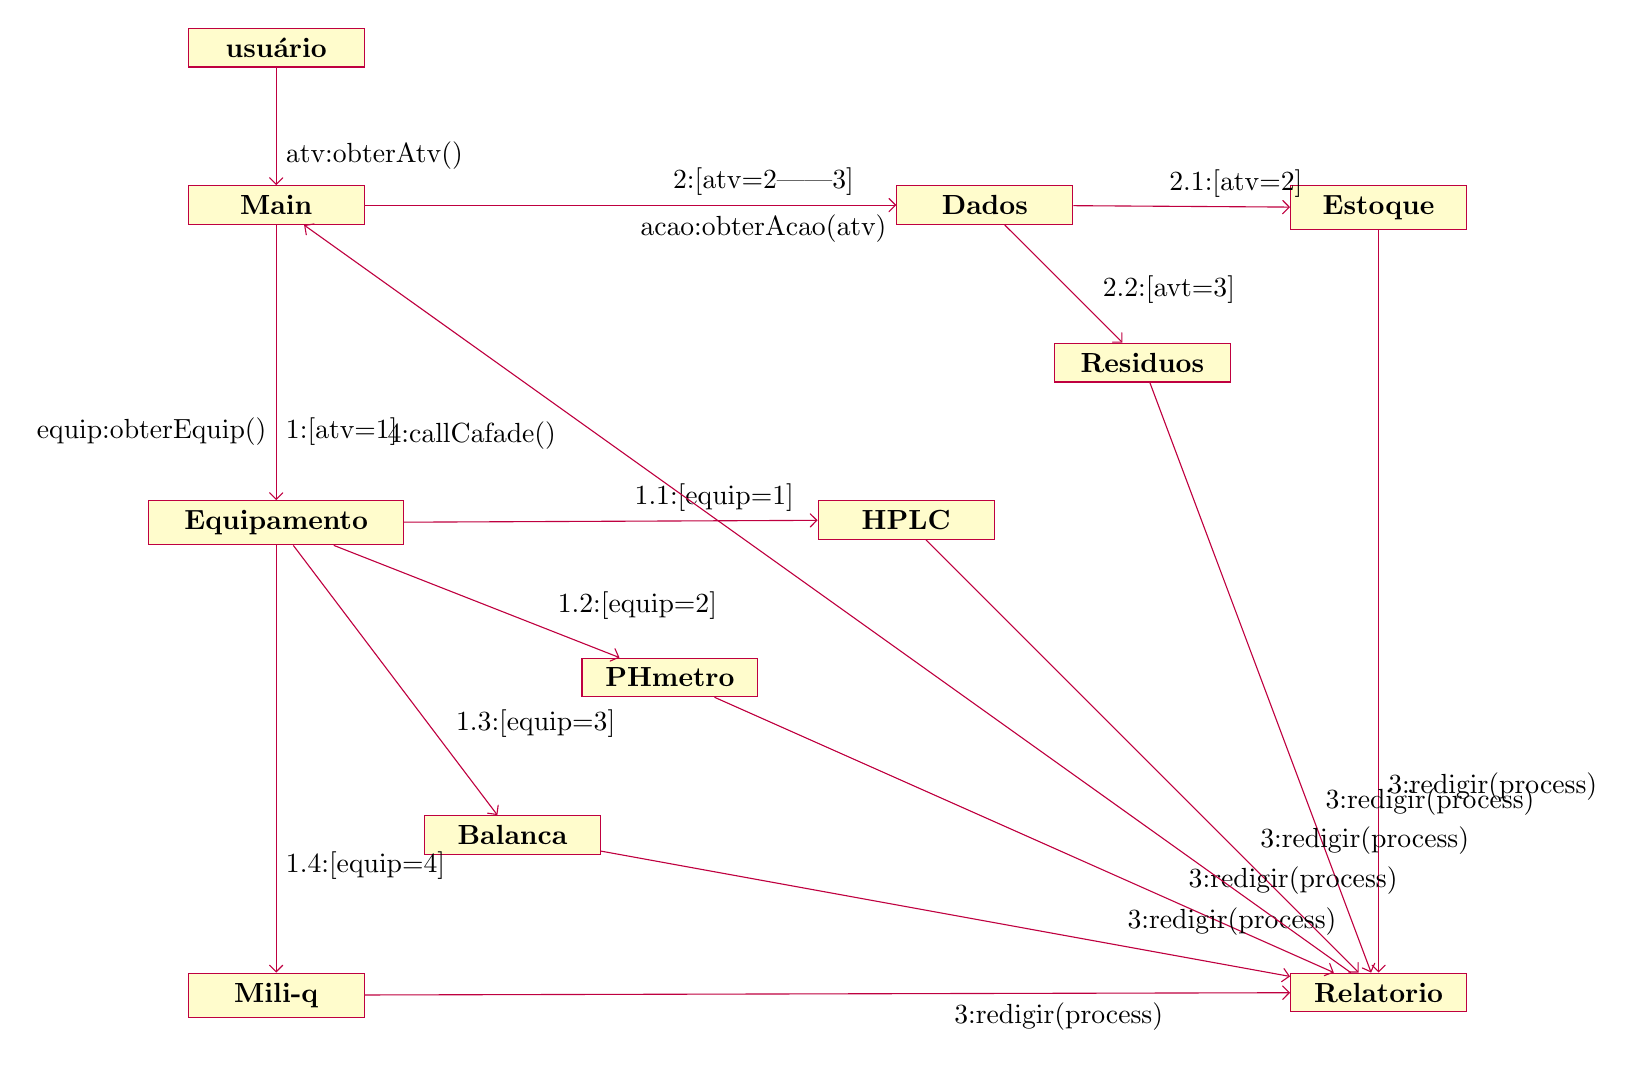
\begin{tikzpicture}
          \begin{class}[text width=2cm]{usuário}{0,0}
          \end{class}
    
          \begin{class}[text width=2cm]{Main}{0,-2}
          \end{class}    
          \unidirectionalAssociation{usuário}{atv:obterAtv()}{}{Main}
    
          %Calibramento de equipamentos
          \begin{class}[text width=3cm]{Equipamento}{0,-6}
          \end{class}
          \unidirectionalAssociation{Main}{1:[atv=1]}{equip:obterEquip()}{Equipamento}
    
            %HPLC
            \begin{class}[text width=2cm]{HPLC}{8,-6}
            \end{class}
            \unidirectionalAssociation{Equipamento}{1.1:[equip=1]}{}{HPLC}
            %PHmetro
            \begin{class}[text width=2cm]{PHmetro}{5,-8}
            \end{class}
            \unidirectionalAssociation{Equipamento}{1.2:[equip=2]}{}{PHmetro}
            %Balança
            \begin{class}[text width=2cm]{Balanca}{3,-10}
            \end{class}
            \unidirectionalAssociation{Equipamento}{1.3:[equip=3]}{}{Balanca}
            %Mili-q
            \begin{class}[text width=2cm]{Mili-q}{0,-12}
            \end{class}
            \unidirectionalAssociation{Equipamento}{1.4:[equip=4]}{}{Mili-q}  
          
          %Requisição de ações
          \begin{class}[text width=2cm]{Dados}{9,-2}
          \end{class}
          \unidirectionalAssociation{Main}{2:[atv=2||3]}{acao:obterAcao(atv)}{Dados}
    
            %Acesso a estoques
            \begin{class}[text width=2cm]{Estoque}{14,-2}
            \end{class}
            \unidirectionalAssociation{Dados}{2.1:[atv=2]}{}{Estoque}
    
            %Gerenciamento de resíduos
            \begin{class}[text width=2cm]{Residuos}{11,-4}
            \end{class}
            \unidirectionalAssociation{Dados}{2.2:[avt=3]}{}{Residuos}
      
          %Relatório  
          \begin{class}[text width=2cm]{Relatorio}{14,-12}
          \end{class}
          \unidirectionalAssociation{Estoque}{3:redigir(process)}{}{Relatorio}
          \unidirectionalAssociation{Residuos}{3:redigir(process)}{}{Relatorio}
          \unidirectionalAssociation{HPLC}{3:redigir(process)}{}{Relatorio}
          \unidirectionalAssociation{PHmetro}{3:redigir(process)}{}{Relatorio}
          \unidirectionalAssociation{Balanca}{3:redigir(process)}{}{Relatorio}
          \unidirectionalAssociation{Mili-q}{}{3:redigir(process)}{Relatorio}
          \unidirectionalAssociation{Relatorio}{4:callCafade()}{}{Main}
        \end{tikzpicture}
      
      \subsubsection{Diagrama de classes}
        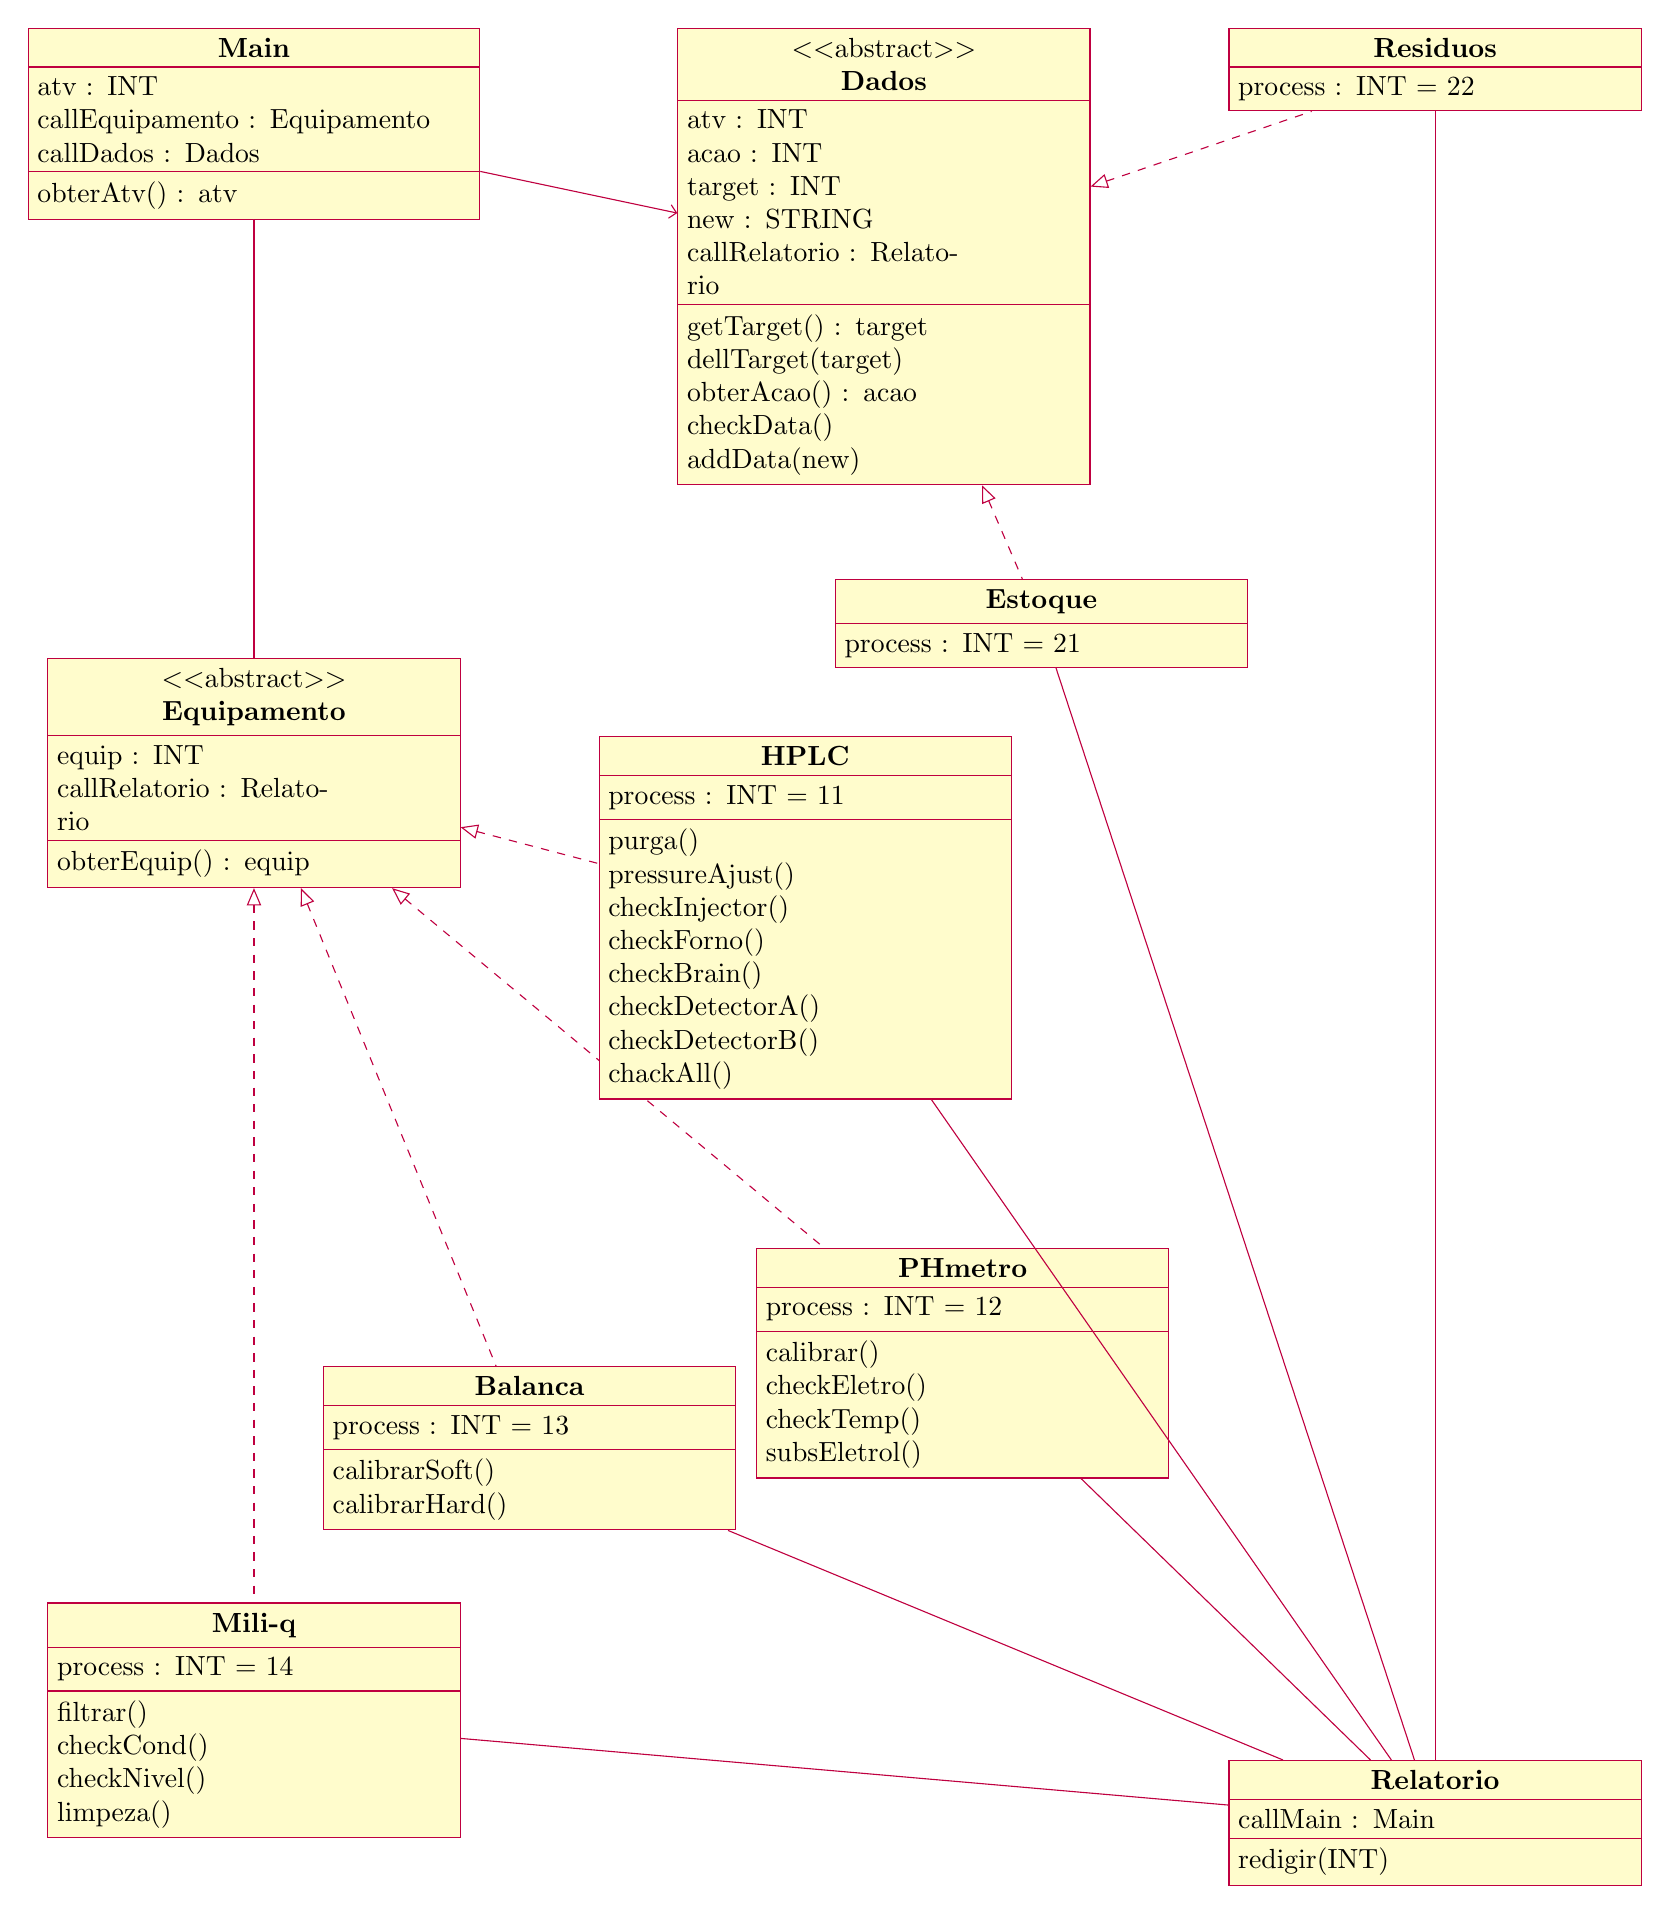
\begin{tikzpicture}
          %Main
          \begin{class}[text width=5.5cm]{Main}{0,0}
            \attribute{atv : INT}
            \attribute{callEquipamento : Equipamento}
            \attribute{callDados : Dados}
            \operation{obterAtv() : atv}
          \end{class}
          %Dados
          \begin{abstractclass}{Dados}{8,0}
            \attribute{atv : INT}
            \attribute{acao : INT}
            \attribute{target : INT}
            \attribute{new : STRING}
            \operation{getTarget() : target}
            \operation{dellTarget(target)}
            \operation{obterAcao() : acao}
            \operation{checkData()}
            \operation{addData(new)}
            \attribute{callRelatorio : Relatorio}
          \end{abstractclass}
          \unidirectionalAssociation{Main}{}{}{Dados}
          %Estoque
          \begin{class}[text width=5cm]{Estoque}{10,-7}
            \implement{Dados}
            \attribute{process : INT = 21}
          \end{class}
          %Resíduos
          \begin{class}[text width=5cm]{Residuos}{15,0}
            \implement{Dados}
            \attribute{process : INT = 22}
          \end{class}
          %Equipamento
          \begin{abstractclass}{Equipamento}{0,-8}
            \attribute{equip : INT}
            \attribute{callRelatorio : Relatorio}
            \operation{obterEquip() : equip}
          \end{abstractclass}
          \association{Main}{}{}{Equipamento}{}{}
          %HPLC
          \begin{class}{HPLC}{7,-9}
            \implement{Equipamento}
            \attribute{process : INT = 11}
            \operation{purga()}
            \operation{pressureAjust()}
            \operation{checkInjector()}
            \operation{checkForno()}
            \operation{checkBrain()}
            \operation{checkDetectorA()}
            \operation{checkDetectorB()}
            \operation{chackAll()}
          \end{class}
          
          %PHmetro
          \begin{class}{PHmetro}{9,-15.5}
            \implement{Equipamento}
            \attribute{process : INT = 12}
            \operation{calibrar()}
            \operation{checkEletro()}
            \operation{checkTemp()}
            \operation{subsEletrol()}
          \end{class}
          
          %Balança
          \begin{class}{Balanca}{3.5,-17}
            \attribute{process : INT = 13}
            \operation{calibrarSoft()}
            \operation{calibrarHard()}
            \implement{Equipamento}
          \end{class}
          
          %Mili-q
          \begin{class}{Mili-q}{0,-20}
            \attribute{process : INT = 14}
            \operation{filtrar()}
            \operation{checkCond()}
            \operation{checkNivel()}
            \operation{limpeza()}
            \implement{Equipamento}
          \end{class}
          
          %Relatório
          \begin{class}{Relatorio}{15,-22}
            \operation{redigir(INT)}
            \attribute{callMain : Main}
          \end{class}
          \association{Estoque}{}{}{Relatorio}{}{}
          \association{Residuos}{}{}{Relatorio}{}{}
          \association{HPLC}{}{}{Relatorio}{}{}
          \association{PHmetro}{}{}{Relatorio}{}{}
          \association{Balanca}{}{}{Relatorio}{}{}
          \association{Mili-q}{}{}{Relatorio}{}{}
        \end{tikzpicture}
        
    \subsection{Algoritmo da solução computacional}
      \begin{lstlisting}
        Main:
          ...
          Escreva("Selecione uma opção")
          Leia(Atividade)
          Se atividade = 1 então:
            Execute Equipamento:
              equip = 0
              Enquanto equip != 5, execute:
                ...
                Escreva("Selecione uma opção")
                Leia(equip)
                Se equip = 1 então:
                  ...
                  Escreva("O que deseja fazer com o HPLC?")
                  Leia(option)
                  Execute HPLC_option:
                    ...
                    Execute Relatorio:
                      ...
                      Execute Main
                Se equip = 2 então:
                  ...
                  Escreva("O que deseja fazer com o pHmetro?")
                  Leia(option)
                  Execute PHmetro_option:
                    ...
                    Execute Relatorio:
                      ...
                      Execute Main
                Se equip = 3 então:
                  ...
                  Escreva("O que deseja fazer com a Balança?")
                  Leia(option)
                  Execute Balanca_option:
                    ...
                    Execute Raletorio:
                      ...
                      Execute Main
                Se equip = 4 então:
                  Escreva("O que deseja fazer com a Mili-q?")
                  Leia(option)
                  Execute Mili-q_option:
                    ...
                    Execute Relatorio:
                      ...
                      Execute Main
                Se equip = 5 então:
                  Execute Main
              Fim enquanto
          Se atividade = 2 ou 3:
            Execute Dados:
              ...
              Escreva("Qual ação será feita?)
              Leia(acao)
              Se atividade = 2 então:
                Execute Estoque_acao:
                  ...
                  Execute Relatorio:
                    ...
                    Execute Main
              Se atividade = e então:
                Execute Residuos_acao:
                  ...
                  Execute Relatorio:
                    ...
                    Execute Main
          Se não, então:
            Retorne 0
      \end{lstlisting}
    \subsection{Link do código e instruções}
      O código com as demais instruções estão disponíveis em repositório do \href{https://github.com/MafiusKity/SAATLQ/tree/main}{github}
\end{document}
